% Construction : A = (0, 0), D = (2, 0), C = (0, 4,8) — une unité vaut 100 m.
% L'angle droit est en A ; l'hypoténuse est [CD], de longueur 520 m.
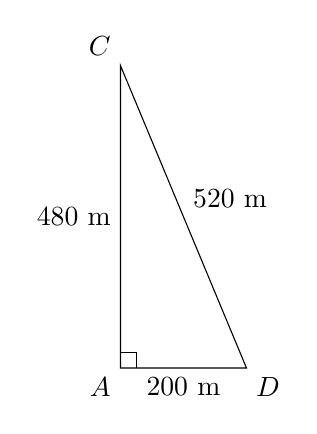
\begin{tikzpicture}[scale=0.8]
  \coordinate (A) at (0, 0);
  \coordinate (D) at (2, 0);
  \coordinate (C) at (0, 4.8);
  \draw (A) -- (D) -- (C) -- cycle;
  \draw (0.25, 0) -- (0.25, 0.25) -- (0, 0.25);
  \node[below left]  at (A) {$A$};
  \node[below right] at (D) {$D$};
  \node[above left]  at (C) {$C$};
  \node[below] at (1, 0)   {$200$ m};
  \node[left]  at (0, 2.4) {$480$ m};
  \node[above right] at (1, 2.4) {$520$ m};
\end{tikzpicture}
